% 1977 年山东A卷第 5 题：△ACD 为正三角形（CD=a，D 左 C 右），A 为炮兵阵地，B 为目标，四点连成带双对角线的四边形（按源卷第 3 页布局）
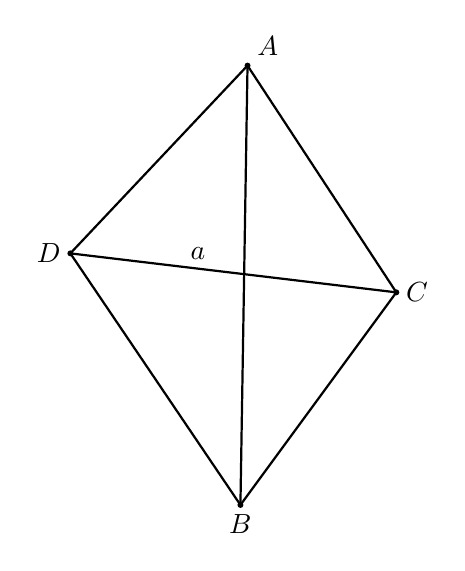
\begin{tikzpicture}[scale=0.9]
  \coordinate (A) at (0.2,3.2);
  \coordinate (D) at (-2.3,0.55);
  \coordinate (C) at (2.3,0);
  \coordinate (B) at (0.1,-3.0);
  \draw[thick] (A) -- (D) -- (C) -- cycle;
  \draw[thick] (A) -- (B);
  \draw[thick] (D) -- (B);
  \draw[thick] (C) -- (B);
  \fill (A) circle (1.2pt) node[above right] {$A$};
  \fill (D) circle (1.2pt) node[left] {$D$};
  \fill (C) circle (1.2pt) node[right] {$C$};
  \fill (B) circle (1.2pt) node[below] {$B$};
  \node at (-0.5,0.55) {$a$};
\end{tikzpicture}
